% !TEX root = Projektspezifikation.tex

\section{Integration}
\subsection{Integrationsprozess}
\subsubsection{Ablauf der Integration}
Für die Integration von weiteren Quellen in die eigene Datenbank werden einige weitere Softwarekomponenten benötigt, um diese einzubinden, dazu zählen eine Downloadmöglichkeit (Skript, o.ä.) und ein lokaler, auf die Quelle zugeschnittener, Parser. Diese müssen dann in den Programmcode an die entsprechende Stelle eingebunden werden. Der lokale Parser wird die heruntergeladenen Dateien entpacken, entschlüsseln und in einem einheitlichen Format abspeichern. Die weiteren Schritte danach wird der feste, globale Parser übernehmen, den man nicht modifizieren muss. Er wird aus den Endprodukten der lokalen Parser die Datensätze rauslesen und diese dann in der Datenbank abspeichern.
\subsubsection{Quellenauswahl}
Unsere derzeitig benutzten Quellen werden die dbSNP und das 1000GenomeProject sein. Die HGMD werden wir nicht benutzen können, da diese Quelle ein Entgelt zur Benutzung der Daten verlangt, was unser Budget übersteigt. Die TCGA Datenbank werden wir vorerst nicht nicht beachten, da uns derzeit noch nicht klar ist, ob deren Daten verwendbar sind. Zu einem späteren Zeitpunkt, wenn die Integration von dbSNP und 1000GenomeProject abgeschlossen ist, werden wir uns mit TCGA befassen und, sollten die Daten erreichbar und verwendbar sein, werden wir diese nehmen um den Erweiterbarkeitsprozess zu verdeutlichen.
\subsubsection{Attributauswahl und -mapping}
Unsere verwendeten Datenbanken stellen uns die Mutationsdaten in .vcf-Dateien bereit. Die Metadaten sind in seperaten .txt-Dateien abgespeichert. Für die Metadaten werden uns die Daten Gender und Population bereitgestellt. Für die Mutation sind die relevanten Daten das Chromosom, in dem die Mutation auftaucht, die Position der Mutation im jeweiligen Chromosom und die vollständige Mutationssequenz. Mit diesen Daten werden wir auch im Weiteren arbeiten. Die Referenzgenome werden in einer separaten Datei abgespeichert, da diese sich nie verändern, und somit ein schnellerer Zugriff auf die Daten gewährleistet wird, und auch ein schnellerer Aufbau der Datenbank selber.
\subsubsection{Mengengerüst}
Der derzeitige Stand des benötigten Speichers beläuft sich auf einige hundert (aber weniger als 500) Gigabyte. Diese Angabe gilt nur für dbSNP und 1000GenomeProject, weitere Quellen werden dementsprechend mehr Speicher benötigen. Weitere Mengenangaben können wir derzeit noch nicht genau machen, diese werden im weiteren Verlauf konkreter und können dann gemacht werden.
\subsubsection{Inputfile-Format}
Referenzgenomname:„Name des Referenzgenoms Bsp: GRCh38“\\
Quelle:„hier die Quelle angeben“\\
\$\$\\
SampleID:„hier Samplename“\\
Genkoordinaten:„Angabe der Koordinaten“ \\
Mutationssequenz:„Sequenz“\\
\$\$\\
SampleID:„hier SampleID aus der Datenbank“\\
Gender:„m oder f“\\
Population:„drei Buchstaben bsp: GBR“ \\
EOF\\
\subsubsection{Sequenzdiagramm}
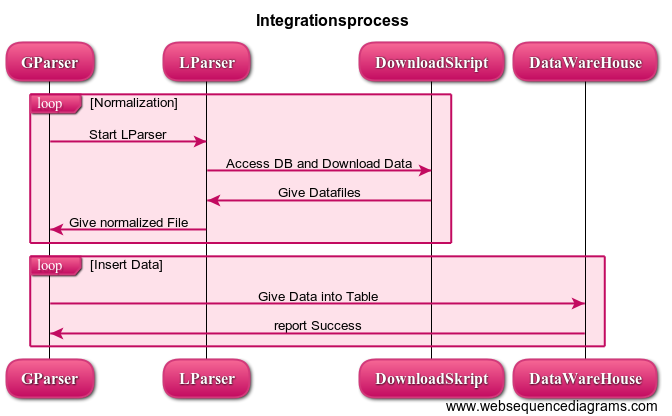
\includegraphics[width=\textwidth]{integration/SQDiag.png}
\subsection{Datenbankentwurf}
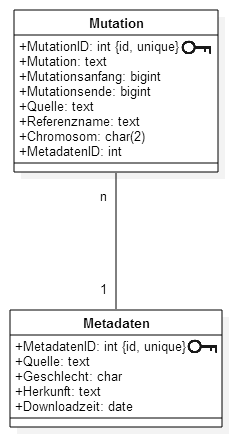
\includegraphics[width=0.5\textwidth]{integration/DB.png}
\subsection{Entwurf des Parsers}
Der lokale Parser wird auf die jeweilige Quelle zugeschnitten sein. Er wird die vorher heruntergeladenen Dateien entpacken, entschlüsseln und danach die relevanten Daten aus den Dateien herauslesen und in einem einheitlichen Format für den globalen Parser abspeichern.\\
Der globale Parser wird die Einheitsdateien der lokalen Parser nehmen, die beinhaltenden Daten in einzelne Datensätze aufteilen und diese dann in der Datenbank abspeichern und sie somit der Middleware bereitstellen.
\subsection{Klassendigramm}
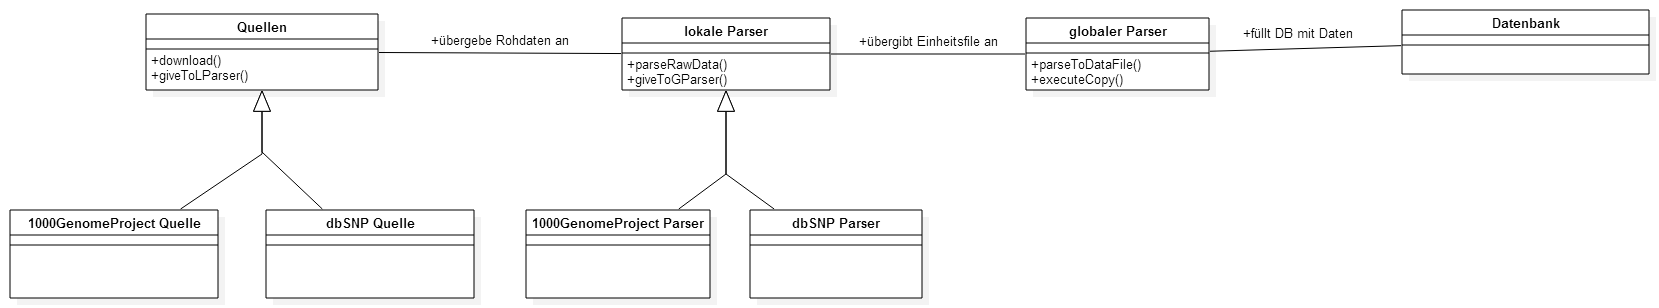
\includegraphics[width=\textwidth]{integration/Klassendiagramm.png}
\subsection{Schnittstellenspezifikation}
\subsubsection{Schnittstelle: Integration - Middleware}
Die Schnittstelle zwischen der Integration und der Middleware ist die, im Modell sichtbare, Datenbank. Sie ist der Ort, an dem die Integration die Daten bereitstellt und von wo die Middleware sich die Daten für die Anfragen abholt.
\subsubsection{Schnittstelle: Integration - Benutzer}
Die Schnittstelle zwischen der Integration und dem Benutzer ist das Hinzufügen neuer Quellen. Der Nutzer wird angehalten sein, zu wissen, wie seine neue Quelle aufgebaut ist, da er selber ein Downloadskript o.ä. dafür schreiben muss, sowie einen lokalen Parser. Diese werden an den entsprechenden Stellen im Programmcode eingefügt. Die lokalen Parser werden durch ein Interface vereinheitlicht.
\subsection{Tests}
\subsubsection{Unit-Tests}
Konkrete Tests konnten wir bisher nicht durchführen, jedoch gibt es einige Dinge zu testen: Es muss getestet werden, ob der lokale Parser arbeitet wie gewünscht, also mindestens 2 Testläufe für ihn: Bei einem, für ihn korrekten Inputfile, muss er ein entsprechend richtiges Outputfile für den globalen Parser erstellen. Sollte er ein Inputfile parsen, was nicht für ihn gedacht ist, soll er das Inputfile verwerfen oder eine Fehlermeldung ausgeben, aber auf alle Fälle das Outputfile nicht mit diesem Input erweitern. Natürlich kann das Inputfile auf verschiedene Weisen korrupt sein, was dort mehrere Testfälle notwendig macht.\\
Der globale Parser muss auf ähnliche Weisen getestet werden, jedoch kann man bei ihm als Voraussetzung annehmen, dass die lokalen Parser korrekt arbeiten und auch ein korrektes Outputfile erstellt haben. Somit müsste nur überprüft werden, dass der globale Parser die Daten korrekt ausliest und korrekt in die Datenbank einfügt.\\
\\
\textbf{Korrektes Inputfile:}\\
\\
Referenzgenomname:GRCh38\\
Quelle:1000Genom\\
\$\$
SampelID:HG0094\\
Genkoordinaten:6:19:19\\
Mutationssequenz: AGTCTAGTA\\
\$\$
SampelID:HG0094\\
Gender:m\\
Population:GRB\\
Download:01:01:2001\\
\\
\textbf{Fehlerhaftes Inputfile}\\
\\
Referenzgenomname:KeinFehlerMöglich\\
Quelle:KeinFehlerMöglich\\
\$\\
SapelID:KeinFehlerMöglich\\
Genkoordinaten:67:21:15\\
Mutationsequenz:ATCERROR\\
\$\$\\
SampelID:KeinFehlerMöglich?\\
Gender:h\\
Population:XXXX\\
Download:64:64:2045\\
